\documentclass{report}
\usepackage{pgf}
\usepackage{tikz}
\usepackage{verbatim}
\usepackage{url}
\usepackage{hyperref}	% Clickable links to figures, references and urls.

\usepackage{graphicx}

\begin{document}

\title{Automated Worm Fingerprinting}
\author{Awais Aslam \and Attique Dawood}
\maketitle

\tableofcontents
\listoffigures

\begin{abstract}
Worms propagate by contacting vulnerable hosts and infecting them with malicious payload.
The destination address space for such attacks would be large. In case of a worm outbreak
number of infected hosts will grow over time. Some part of worm attack patterns are always
invariant. Such invariant content can be used as worm signatures by analyzing the frequency
at which this content appears in network traffic and the variance in source and destination
addresses. We present an implementation of this method for detecting worms based on the
EarlyBird prototype~\cite{DBLP:conf/osdi/SinghEVS04}.
\end{abstract}

\chapter{Introduction}
\section{Network Intrusion Detection Systems}

Intrusion detection systems monitor network traffic to detect malicious activities. Malicious activities can be an outside attempt to gain control of a host, a worm spreading across the internet or suspicious traffic from a local host etc.

\section{Types of IDS}

IDS are basically either signature--based or anomaly--based. Signature--based IDS need to know specific signatures of malicious content (specific strings or code) beforehand. Anomaly--based IDS identify abnormal patterns in network traffic for detecting suspicious activities.

\section{Automated Signature Generation}

Sumeet et. al.~\cite{DBLP:conf/osdi/SinghEVS04} have presented a method to quickly generate signatures based on anomalous behaviour of worms spreading across the network in order contain them. The method is based on an observation that the probability of unique strings occurring in normal traffic directed to diverse destination is very low.

Intrusion detection techniques used by Snort and Bro rely on vulnerabilities that are well--known by comparing with a database. Automated worm detection assumes that some part of malicious program or code is invariant, i.e. it does not change in order to hide itself. The invariant portion of worm can be used to create signatures since it will occur frequently in network traffic.

The goal of this project is to come up with an efficient implementation of the signature generation algorithm used in EarlyBird prototype.

\chapter{Problem Specification}

\section{Characterizing Worm Behaviour}
Worms are defined as malicious programs that can replicate and spread over the network infecting vulnerable hosts.

Observation of popular worm outbreaks reveal that spreading rate is extremely fast. For example the Slammer worm scanned almost all the internet address space in under 10 minutes~\cite{DBLP:conf/osdi/SinghEVS04}. There is a need to quickly generate signatures in case of a new worm outbreak.

\section{Project Goals}
The goals of this project was to implement an automated worm detection software that can quickly generate worm signatures in order to contain worm activities.

The minimum functionality was to detect already existing worms on the network. In addition, real-time analysis of network traffic requires an efficient implementation to reduce the computational overheads. The program should also be flexible to allow changes in operational parameters in order to tune it for best performance and results.

\chapter{Solution Approach}

\section{Algorithm}
Content Prevalence and Address Dispersion tables keep track of content prevalence and content dispersion. Content prevalence table has two fields for key and count. Address dispersion table has three fields for key, source IP count and destination IP count. Following steps outline the core functionality as depicted in figure~\ref{Algorithm} taken from~\cite{DBLP:conf/osdi/SinghEVS04}:
\begin{enumerate}
\item Network traffic is scanned and keys are generated from packet payloads.
\item If the key is already present in address dispersion table relevant source or destination IP count is incremented. Alarm thresholds are checked in this case.
\item If the key doesn't exist in address dispersion table it is checked in Content prevalence table. If present, content prevalence count is incremented otherwise a new entry is created with count 1. 
\item If the content prevalence count crosses threshold, key is promoted into address dispersion table.
\end{enumerate}

\begin{figure}[here]
\centering
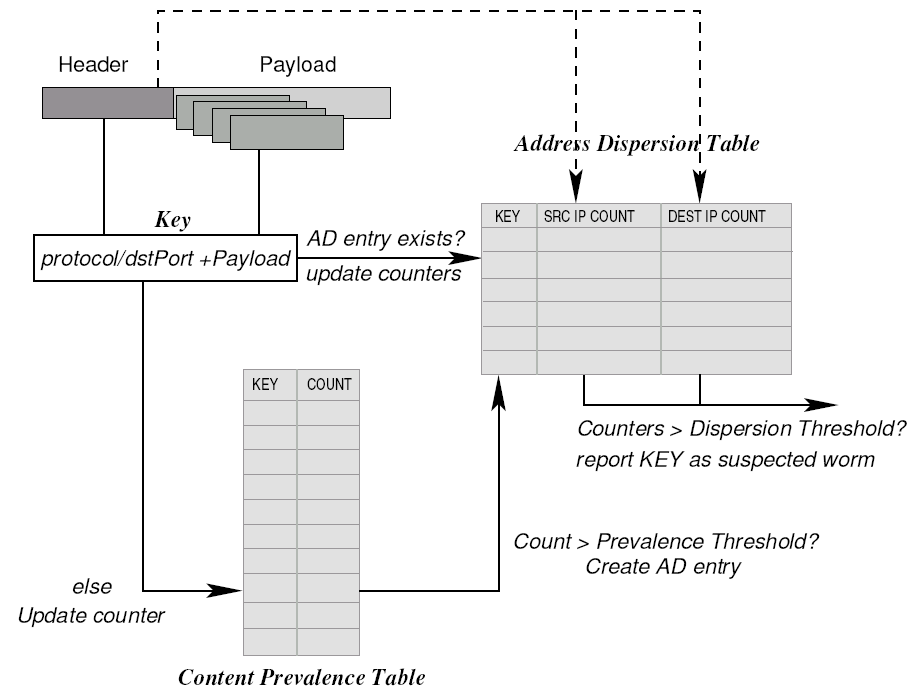
\includegraphics[width=\textwidth]{Algorithm.png}
\caption{Worm detection algorithm}
\label{Algorithm}
\end{figure}

\section{Main Components}
Our implementation is portable and can be run on both Linux or Windows provided the required development libraries are installed. It has the following main components:
\begin{enumerate}
\item Packet capturing section that provides packet payload and header information
\item Packet processing thread to generated keys and index into Content Prevalence and Address Dispersion tables.
\item A garbage collector thread removes any keys from content prevalence table that are outdated.
\item Another thread logs network statistics and dumps any debugging information requested by user.
\end{enumerate}

\chapter{Implementation Details}

\section{Packet Capturing}
On Linux we used the \texttt{libpcap} and for Windows we used the \texttt{winpcap} packet capturing libraries. These libraries are open source projects freely available online.

A filter string needs to be passed as an input argument to the software. This filter string specifies the network traffic to capture. For example, using a filter string ``ip'' will capture all IP packets, similarly a filter string ``TCP\textbar\textbar UDP'' will capture any TCP or UDP packets.

\section{Key Generation}
Keys are hashes generated from sub-strings of packet payload. Use can choose from several hashing techniques. A comparison of computational requirements of different hashing schemes is given in figure~\ref{HashingSchemes}. Following hashing schemes can be used with our implementation:
\begin{enumerate}
\item Rabin 32 bit
\item Interleaved Rabin 32 bit
\item Rabin 64 bit
\item Interleaved Rabin 64 bit
\item MD5
\item SHA1
\end{enumerate}

\begin{figure}[here]
\centering
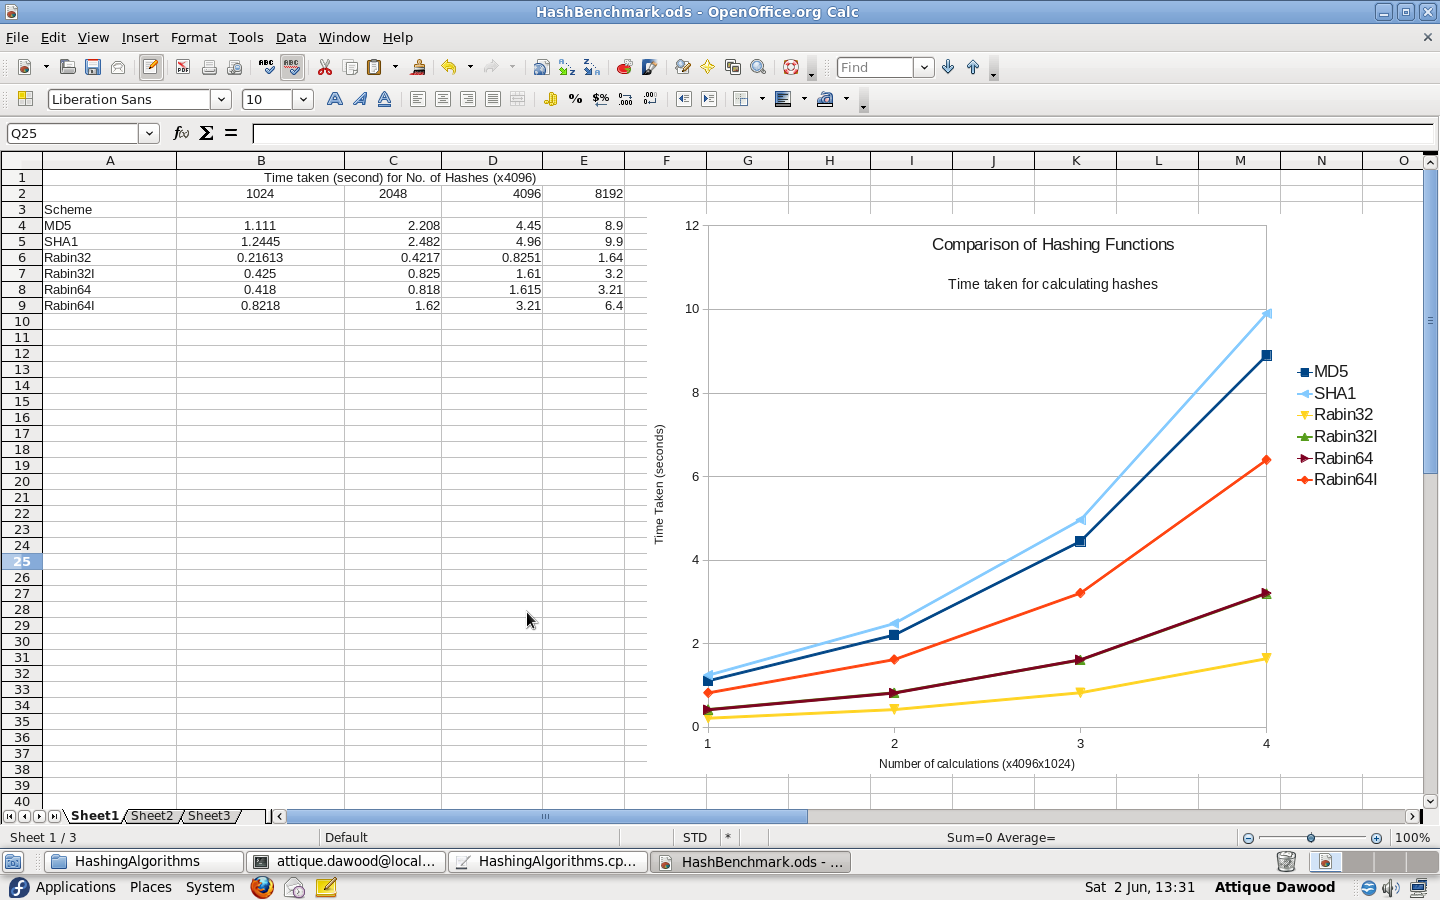
\includegraphics[width=\textwidth]{HashingSchemes.png}
\caption{Comparison of hashing schemes}
\label{HashingSchemes}
\end{figure}

\section{Content Prevalence and Address Dispersion Tables}
The Content Prevalence Table is a hash map of entries with following structure:
\begin{verbatim}
struct ContentPrevalenceEntry
{
    int Count;
    __int64 InsertionTime;
};
map<vector<unsigned char>, ContentPrevalenceEntry> ContentPrevalenceTable;
\end{verbatim}

Similarly the Content Prevalence Table is a hash map of entries with following structure:
\begin{verbatim}
struct AddressDispersionEntry
{
    vector<in_addr> SrcIPs;
    vector<unsigned short> SrcPorts;
    vector<in_addr> DstIPs;
    vector<unsigned short> DstPorts;
    int AlarmCount;
};
map<vector<unsigned char>, AddressDispersionEntry> AddressDispersionTable;
\end{verbatim}

Using map has the advantage that searching and insertion takes $O(log(n))$ compared to $O(n)$ time taken by array or vector. We used both implementations and observed a marked increase in performance when using map compared to vector (figure~\ref{MapVsVector}). The one on left is that of vector while on the right is map implementation.

\begin{figure}[here]
\centering
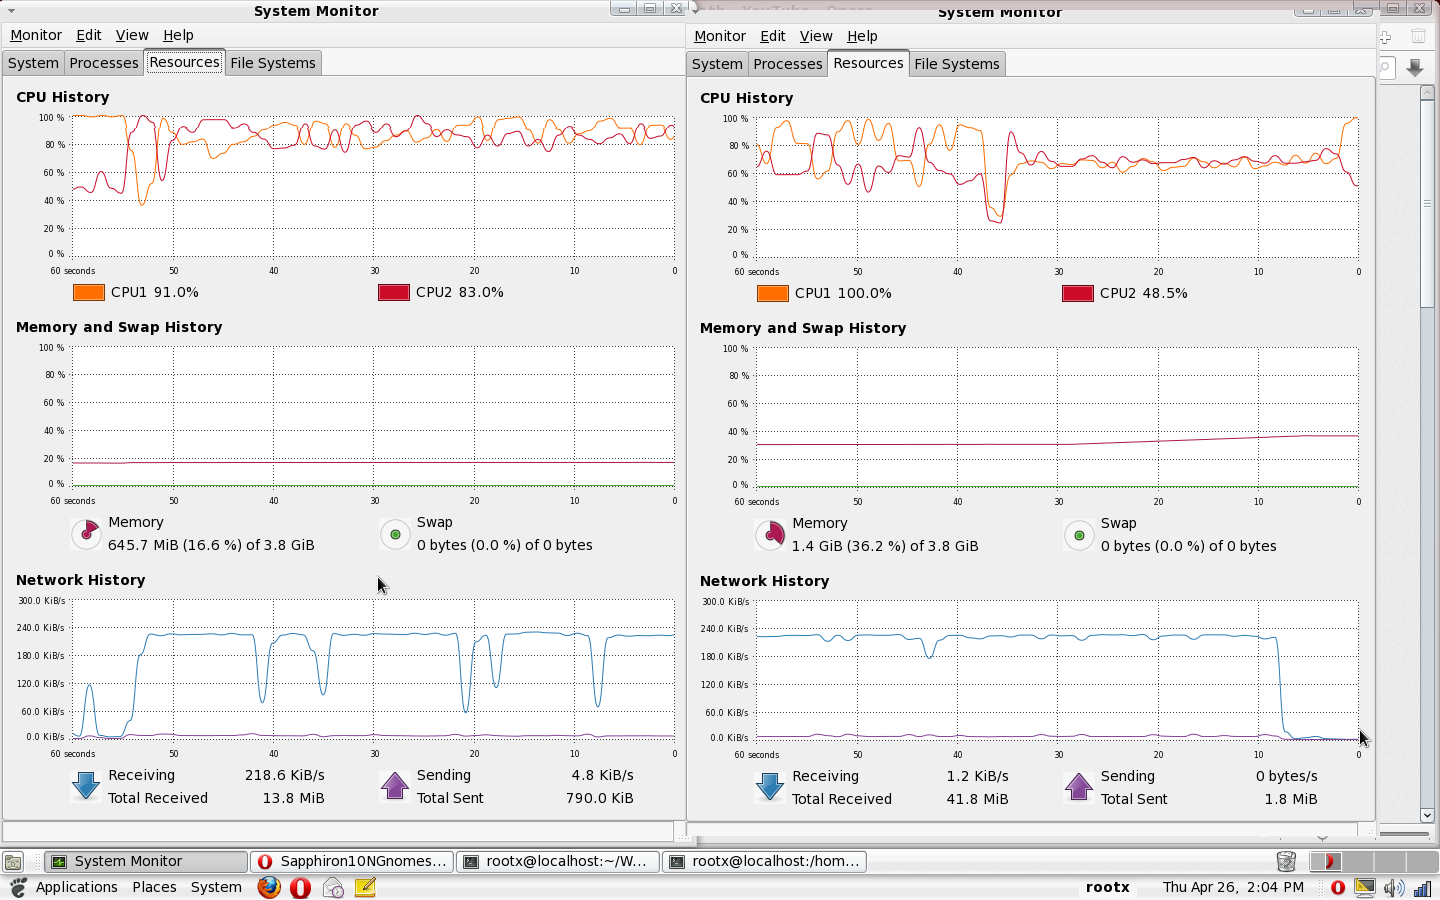
\includegraphics[width=\textwidth]{MapVsVector.png}
\caption{Map vs vector performance}
\label{MapVsVector}
\end{figure}

The first entry in both maps is the key implemented as a vector of type \texttt{unsigned char}. The address dispersion table not only keeps track of number of unique source and destination IPs but also source and destination ports. Alarm count is incremented by one every time a unique source or destination IP is inserted. Alarm is raised if the source and destination IP vectors exceed the set thresholds called address dispersion thresholds.

\section{Garbage Collection}
Garbage collection is extremely important to efficient functioning of this software. Every time keys are generated, they are searched in the content prevalence and address dispersion tables. Size of content prevalence table is important because larger tables will result in longer search times.

It is observed that most of the keys in the content prevalence table never occur more than once. Therefore, keys with prevalence count of 1 are deleted after a set time-out interval. If prevalence count is incremented the time-out interval is also reset in order to ensure that prevalent content isn't garbage collected. A garbage collector thread is invoked after a set interval. This interval can be adjusted by user.

\section{Logging}
User can opt to log network traffic statistics over the course of program execution. There are additional options to log host-specific and port-specific network traffic statistics. Figure~\ref{NetworkStats} shows an example of network statistics logged in a text file.

In addition to network statistics, content prevalence and address dispersion tables are also logged and saved in log files. Example of content prevalence and address dispersion table log files is shown in figures~\ref{ContentPrevalenceLog} and~\ref{AddressDispersionLog}.

\begin{figure}[here]
\centering
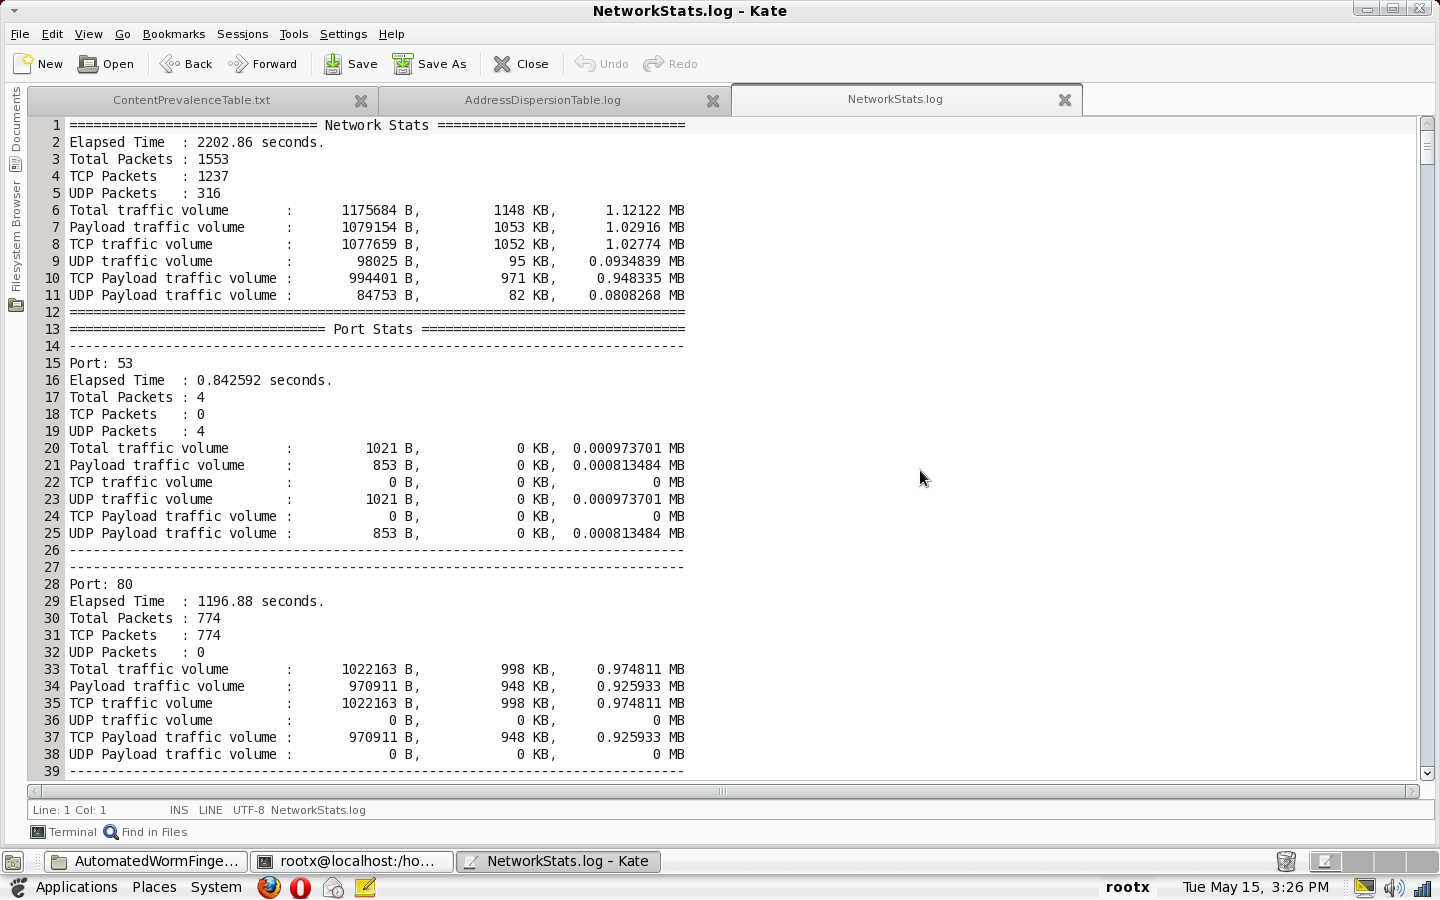
\includegraphics[width=\textwidth]{NetworkStats.png}
\caption{Network statistics}
\label{NetworkStats}
\end{figure}

\begin{figure}[here]
\centering
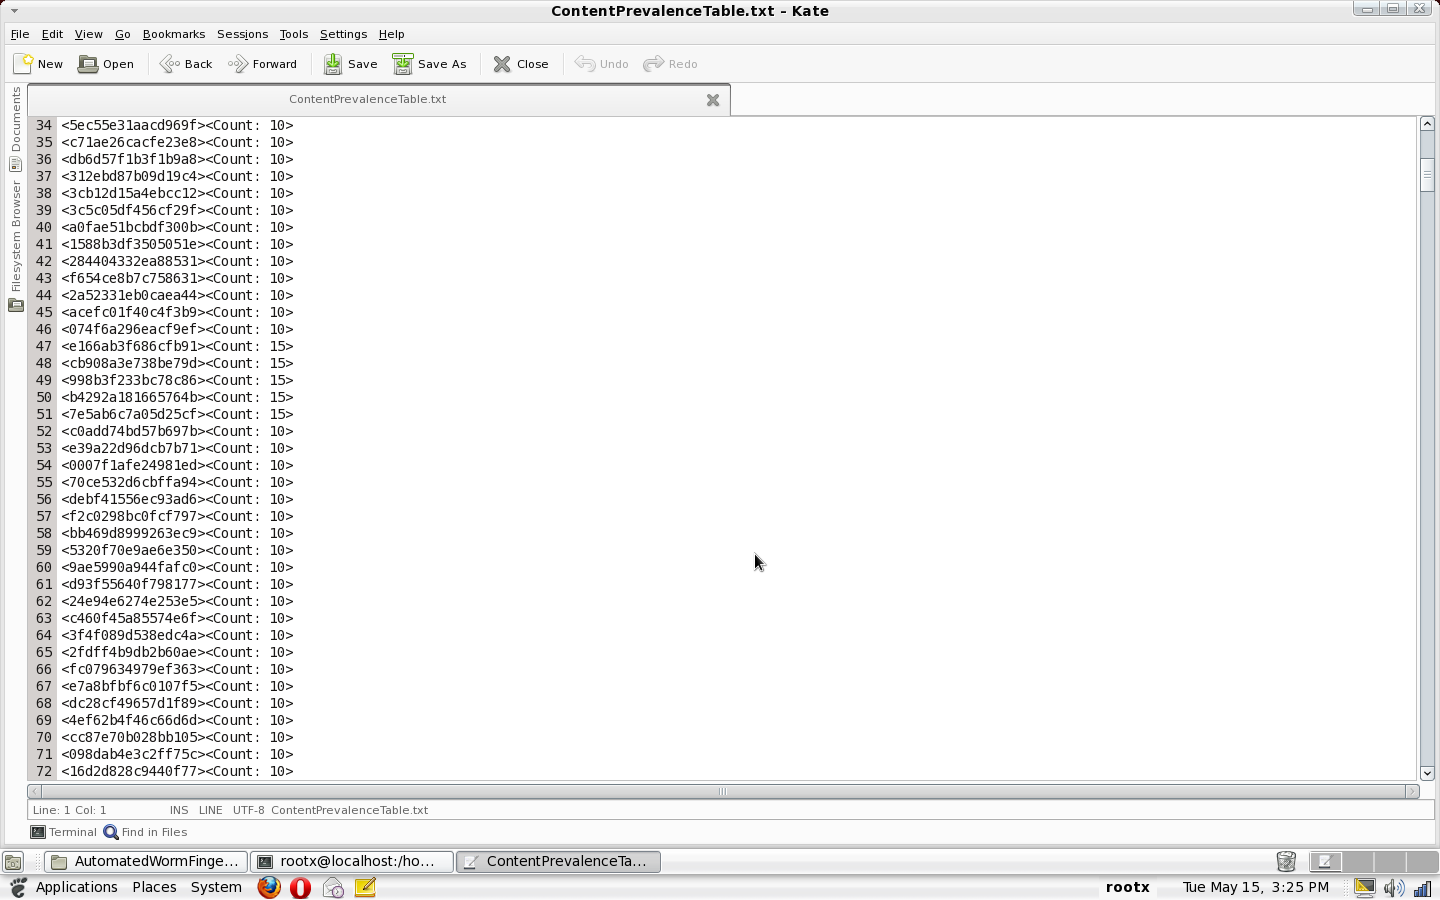
\includegraphics[width=\textwidth]{ContentPrevalenceTable.png}
\caption{Content prevalence table}
\label{ContentPrevalenceLog}
\end{figure}

\begin{figure}[here]
\centering
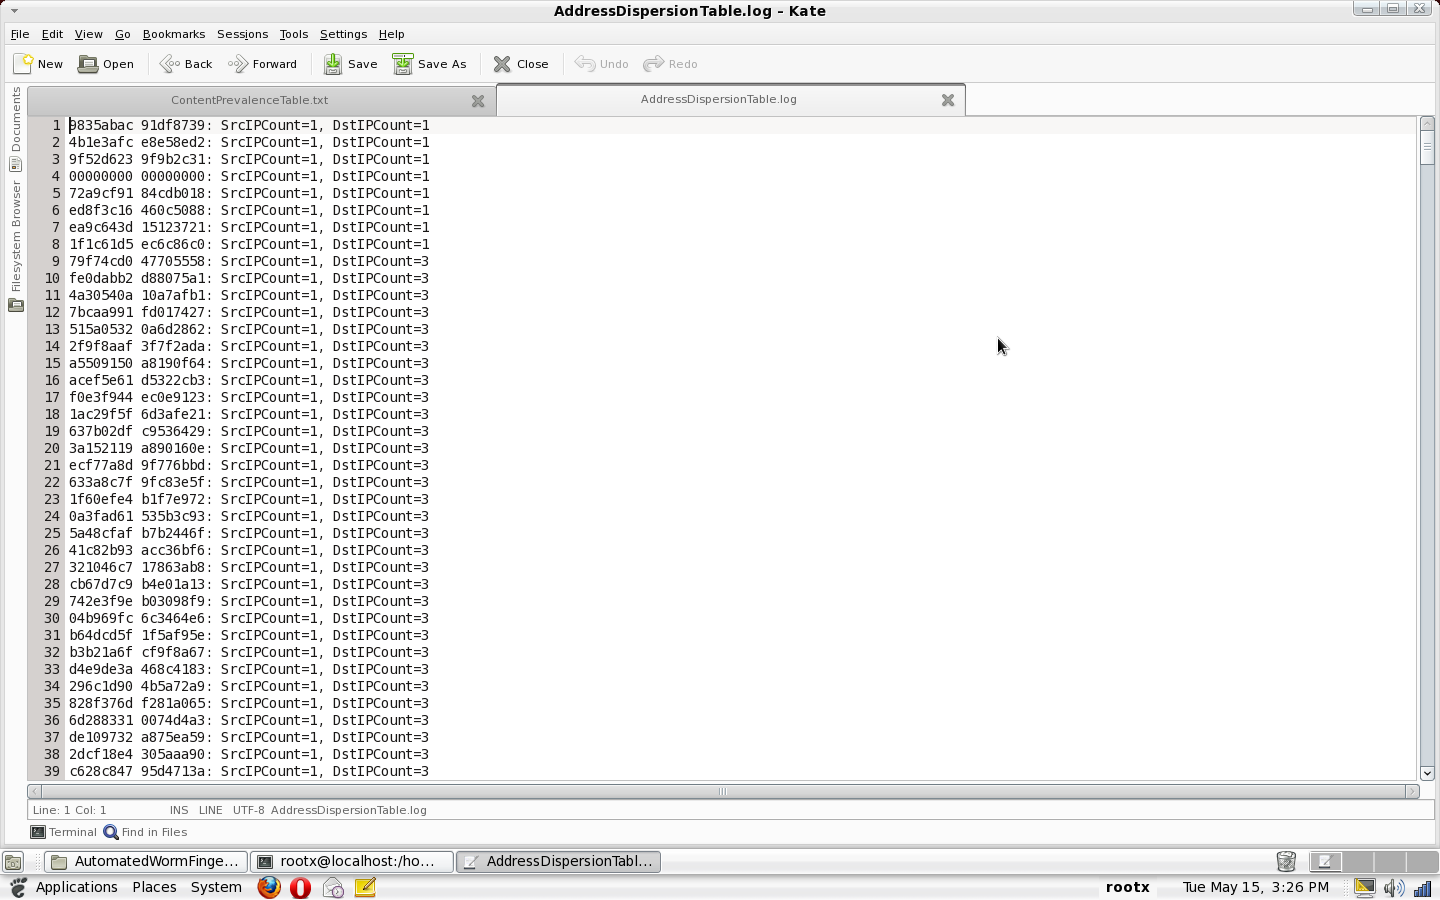
\includegraphics[width=\textwidth]{AddressDispersionTable.png}
\caption{Address dispersion table}
\label{AddressDispersionLog}
\end{figure}

\section{Modes of Operation and Input Arguments}
There are two modes of operation:
\begin{enumerate}
\item Server Mode
\item Client Mode
\end{enumerate}

When running in server mode all the processing is done by server including key generation and maintaining content prevalence and address dispersion tables. In client mode only keys or signatures are generated and are then passed to the server for further processing. A client doesn't keep content prevalence or address dispersion tables and only acts as a sniffer or sensor that can capture network traffic.

The client mode of operation offloads some of the processing workload of server by capturing traffic and generating keys. It also has the advantage of acting as a remote sensor when there are multiple distinct streams of traffic flows or different backbones.

The server or client modes are determined by input arguments that are passed when running the program. Server mode requires three input arguments whereas client mode requires five arguments. The mode is determined by the number of arguments.
\begin{enumerate}
\item Interface to sniff on, e.g. \texttt{eth0} or \texttt{wlan0}. On Windows it is better to specify this as \texttt{NULL} and user will asked to select from a list of interfaces.
\item Filter string, e.g. \texttt{TCP}, \texttt{UDP}, texttt{ip} etc. The filter strings can be combined using logical operators.
\item Server port.
\item Client port. (Client only)
\item Server address/IP. (Client only)
\end{enumerate}

\chapter{Experimental Testing and Results}

We carried out our testing in two steps. First we started with an emulated worm to test whether our software was functioning correctly. In next step we carried sniffed real network traffic of one of our labs and detected two potential threats. The simulation parameters are as follows:
\begin{verbatim}
#define SUBSTRING_PROCESSING			1
#define SUBSTRING_WINDOW				32
#define CONTENT_PREVALENCE_TIMEOUT		120.	// seconds
#define CONTENT_PREVALENCE_THRESHOLD	20
#define SRC_IP_DISPERSION_THRESHOLD		5
#define DST_IP_DISPERSION_THRESHOLD		5
#define GARBAGE_COLLECTION_INTERVAL		60		// seconds
#define LOGGING_INTERVAL				30		// seconds
\end{verbatim}

\section{Emulated Vulnerable Server}
We wrote an application that can be considered a vulnerable server. By sending a certain string pattern the server can be 'infected' and will start sending out such string patterns to all the hosts on the subnet. This 'infectious' string can appear as a sub-string in a payload and can be encrypted in five different ways.

By running the vulnerable server on different computers in the lab our software was able to detect suspicious activities that confirmed it was functioning correctly.

\section{Real-time Testing}
In actual testing we found that a number of computers were generating excessive NetBIOS traffic on ports 137 and 138. We identified such behaviour as possible cases of infections by W32.Opaserv on port 137~\ref{Alarm} and W32.Spybot on port 138~\ref{Port138Alarm}. The generated alarm report is shown in figure~\ref{Port137Alarm}.

Analysis of one of the infected computers revealed that system process running on port 138 was taking excessive memory (figure~\ref{Infected138}.

\begin{figure}[here]
\centering
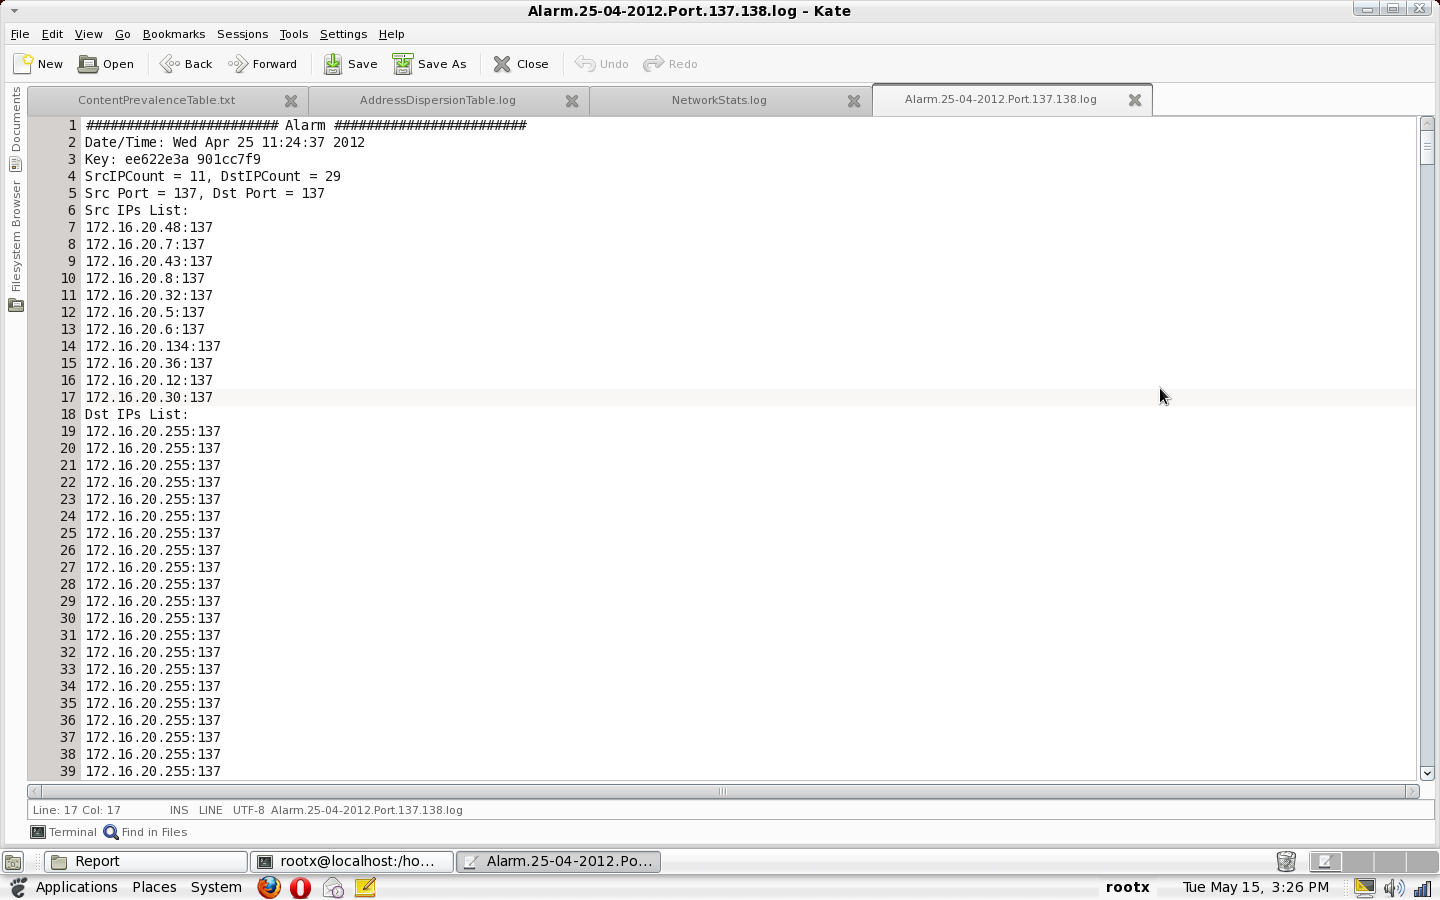
\includegraphics[width=\textwidth]{Port137Alarm.png}
\caption{Alarm showing port 137 is generating suspicious traffic}
\label{Port137Alarm}
\end{figure}

\begin{figure}[here]
\centering
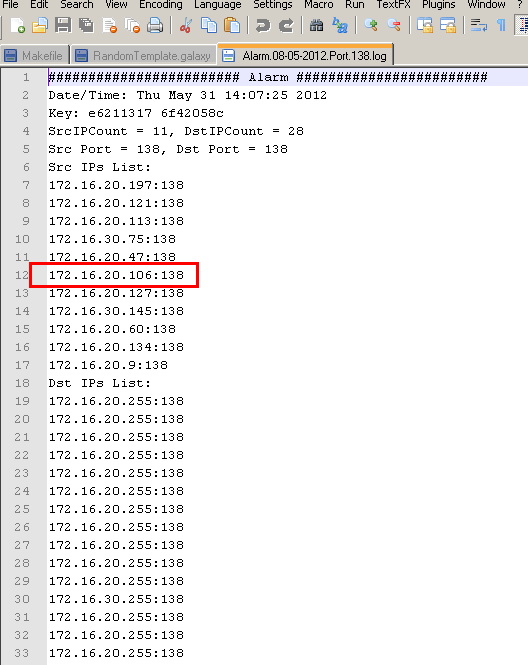
\includegraphics[width=\textwidth]{Port138Alarm.png}
\caption{Alarm showing port 138 is generating suspicious traffic}
\label{Port138Alarm}
\end{figure}

\begin{figure}[here]
\centering
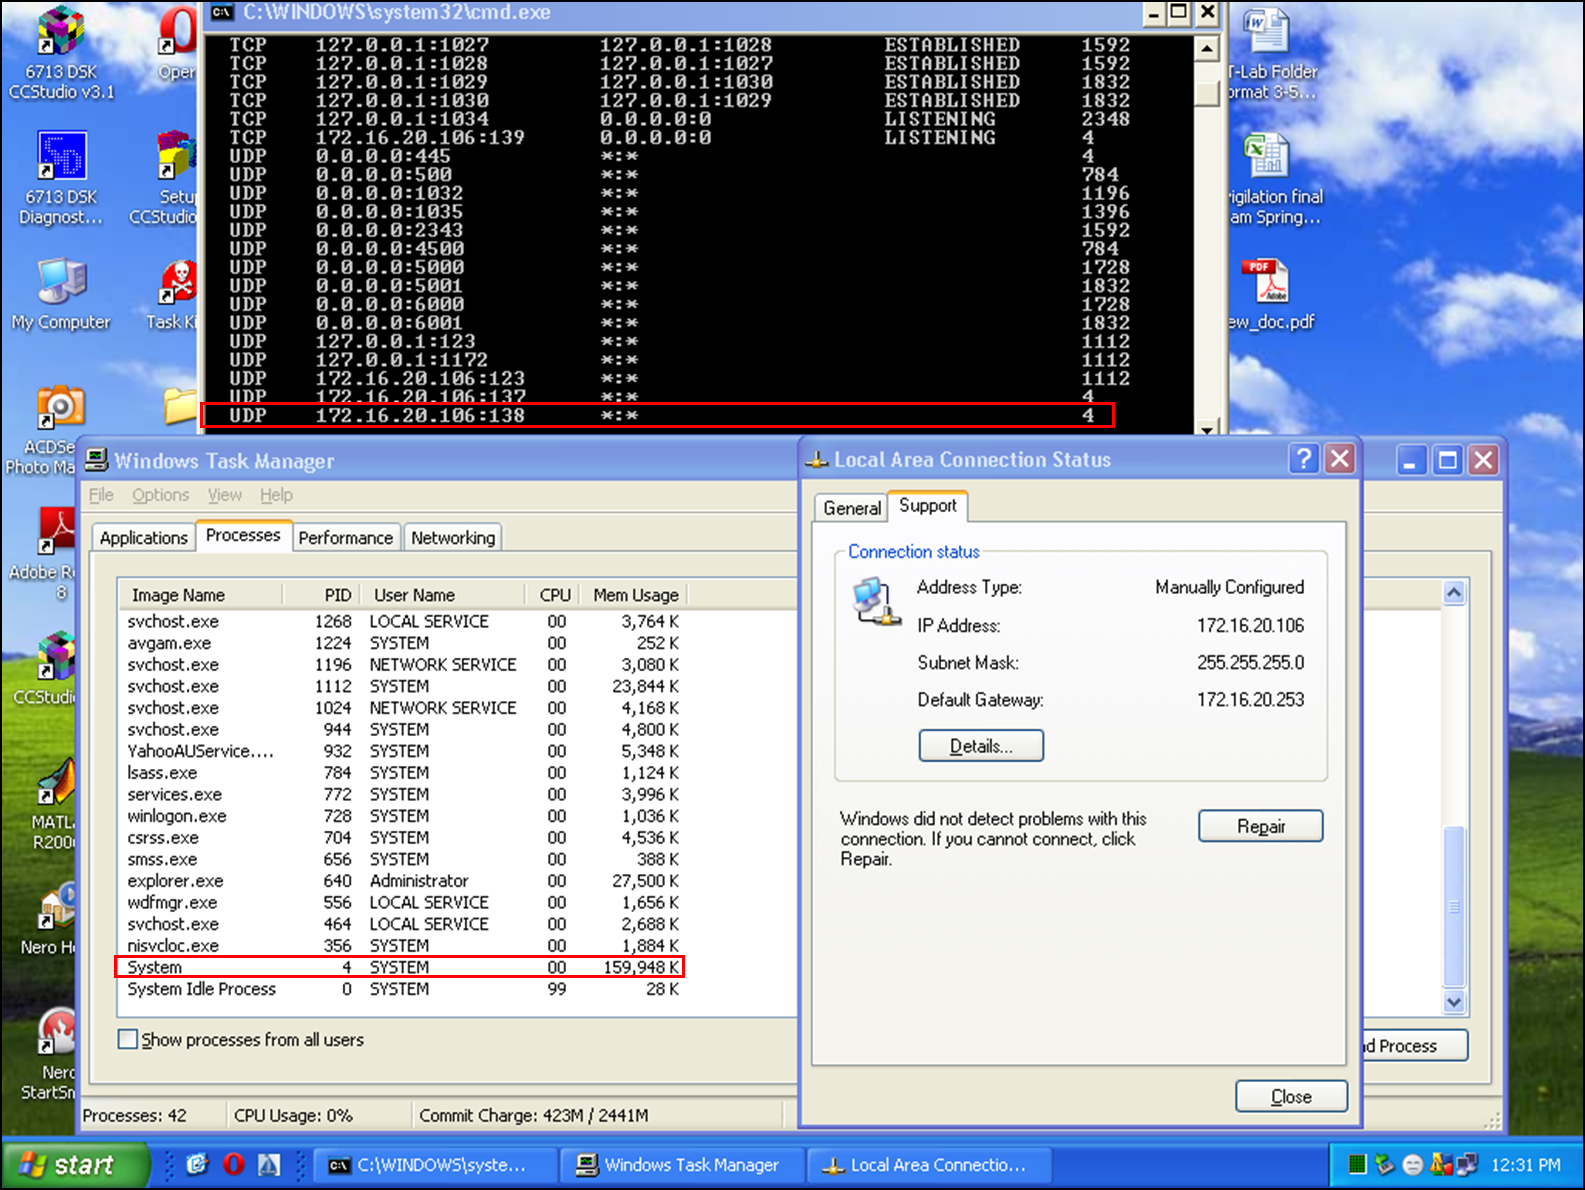
\includegraphics[width=\textwidth]{Port138WindowsSuspicious.png}
\caption{Suspicious activity on port 138}
\label{Infected138}
\end{figure}

\chapter{Further Testing and Improvements}
Our results showed that an automated worm detection program can work in real-time within computational restraints and still manage to effectively detect potential threats. However, there are still further improvements that we suggest in order to make it viable for high bandwidth traffic.
\begin{enumerate}
\item We used the STL container map provided as a standard C++ library in order to utilize the sequential iterators. Boost libraries, however, provide a more efficient hash map that can further improve performance.
\item Garbage collection and prevalence time-out time can be dynamically adjusted as functions of network traffic to further improve CPU overhead.
\item Clients can further reduce the server computational workload by keeping local content prevalence tables. These tables can be exchanged with the server at periodic intervals thereby further reducing server workload.
\end{enumerate}

\nocite{*}
\bibliographystyle{ieeetr} %plain, ieeetr
\bibliography{Wormref}

\end{document}




